\subsection{Hasil Pengujian}

\subsubsection{Iterasi Perbaikan Sistem}
\label{subsubsec:iterasi-perbaikan-sistem}

Terdapat beberapa permasalahan yang ditemukan selama proses implementasi dan pengujian sistem ini, yang kemudian diatasi dengan melakukan iterasi perbaikan sistem. Beberapa permasalahan tersebut antara lain:

\begin{enumerate}
	\item Dgraph UID tidak \textit{stable} yang menyebabkan pengujian tidak dapat dilakukan secara konsisten untuk pelabelan data. Hal ini diatasi dengan menambahkan atribut \texttt{ContractDeployments.id} yang menggunakan atribut sebelum dilakukan \textit{enrichment} dan melakukan \textit{hashing} untuk menjadikan sebuah ID yang unik dan konsisten untuk setiap Smart Contracts. Dengan cara ini, ID tersebut akan tetap konsisten meskipun UID Dgraph berubah.
	\item Proses enrichment yang dilakukan pada data sangat bergantung pada prompt yang diberikan. Hal ini menyebabkan hasil enrichment yang dapat bervariasi. Hal ini diatasi dengan melakukan iterasi pada prompt yang digunakan untuk enrichment, sehingga hasil enrichment dapat lebih konsisten dan relevan dengan data yang ada. Iterasi ini dilakukan dengan mengubah prompt yang digunakan pada proses enrichment dan melakukan pengujian terhadap hasil yang diperoleh.
	\item Proses enrichment berdasarkan \textit{source code} Smart Contract yang dilakukan pada tahap awal tidak memberikan hasil yang optimal karena metode pemotongan yang digunakan. Secara spesifik, source code dari sebuah Smart Contract seringkali memiliki penyusunan urutan yang spesifik, dimulai dari \texttt{library} yang digunakannya terlebih dahulu sehingga mengaburkan konteks keseluruhan jika kontrak tersebut menggunakan banyak \textit{library}. Hal ini diatasi dengan menghilangkan pemotongan token. Dengan cara ini, walau biaya token meningkat, proses enrichment dapat dilakukan dengan lebih baik dan hasil yang diperoleh lebih relevan dengan data yang ada.
	\item Proses enrichment dan retrieval sangat bergantung pada format yang digunakan untuk menyimpan data. Format yang digunakan harus dapat mengakomodasi pencarian semantik yang spesifik. Hal ini diatasi dengan melakukan ekstensi dan juga perubahan atribut, sehingga dapat dengan lebih spesifik mengakomodasi kebutuhan pencarian semantik.
	\item Proses konversi menjadi embeddings membutuhkan konteks penjelasan tambahan terkait istilah-istilah spesifik domain yang digunakan. Hal ini diatasi dengan menambahkan sebuah \textit{dictionary} yang berisi istilah-istilah spesifik domain yang digunakan pada proses enrichment. Dengan cara ini, proses konversi menjadi embeddings dapat dilakukan dengan lebih baik dan hasil yang diperoleh lebih relevan dengan data yang ada. Hasil dari \textit{dictionary} ini dapat dilihat pada Lampiran \ref{appendix:embeddings-dictionary}.
	\item Pengujian membutuhkan fitur tambahan untuk melakukan \textit{benchmarking} terhadap hasil yang didapatkan. Hal ini diatasi dengan menambahkan fitur tambahan pada sistem, terutama pada bagian Dgraph Client, API, dan Web GUI untuk melakukan pencarian berbasis teks kepada Source Code dan juga hasil deskripsi semantik yang dihasilkan. Dengan fitur ini, pengujian \textit{benchmark} dapat dilakukan dengan lebih mudah. Hasil perubahan ini dapat dilihat pada setiap lampiran implementasi.
	% Bisa kasih lampiran, terus juga bilang kalau ini ada tradeoff di token, jadi lebih mahal tapi lebih baik
	% tapi gemini disini dipake karena lebih murah dan lebih besar context windownya
\end{enumerate}

\subsubsection{Pengujian Sistem Pencarian Berbasis Semantik dari Iterasi Awal}

Hasil dari pengujian ini dapat dilihat pada Gambar \ref{image:pengujian-1}. Hasil dari pengujian ini menunjukkan rata-rata presisi sebesar 55\%. Tetapi, terdapat inkonsistensi dari hasil yang diperoleh untuk beberapa query yang diberikan, dimana terdapat query memberikan hasil yang sepenuhnya relevan, tetapi terdapat juga query yang tidak memberikan hasil yang relevan sama sekali. Hal ini menunjukkan bahwa sistem masih perlu diperbaiki, terutama dalam hasil enrichment yang dibaca oleh ahli, dimana deskripsi yang dihasilkan dinilai masih cukup umum, sehingga tidak memberikan hasil yang cukup spesifik.

\begin{figure}[ht]
	\centering
	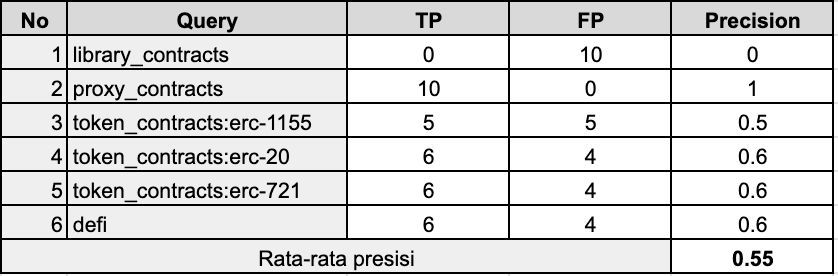
\includegraphics[width=1\textwidth]{resources/chapter-4/data-1-1.png}
	\caption{Hasil Pengujian Sistem Pencarian Berbasis Semantik dari Iterasi Awal}
	\label{image:pengujian-1}
\end{figure}

\subsubsection{Pengujian Sistem Pencarian Berbasis Semantik dari Iterasi Perbaikan dengan Query Bahasa Alami}

Hasil dari pengujian ini dapat dilihat pada Gambar \ref{image:pengujian-2}. Hasil dari pengujian ini menunjukkan rata-rata presisi sebesar 65\%, peningkatan 10\% jika dibandingkan dengan iterasi awal. Hal ini menunjukkan bahwa presisi sistem dipengaruhi oleh mekanisme enrichment yang dilakukan. Selain itu, sistem dapat mendapatkan hasil spesifik dari sebuah kontrak hanya dengan mendeskripsikan isi fungsionalitas atau tujuan dari Smart Contract tersebut. Secara umum, hasil pencarian semantik yang didapatkan cukup konsisten, dimana terdapat hasil-hasil yang relevan untuk setiap query yang diberikan.

\begin{figure}[ht]
	\centering
	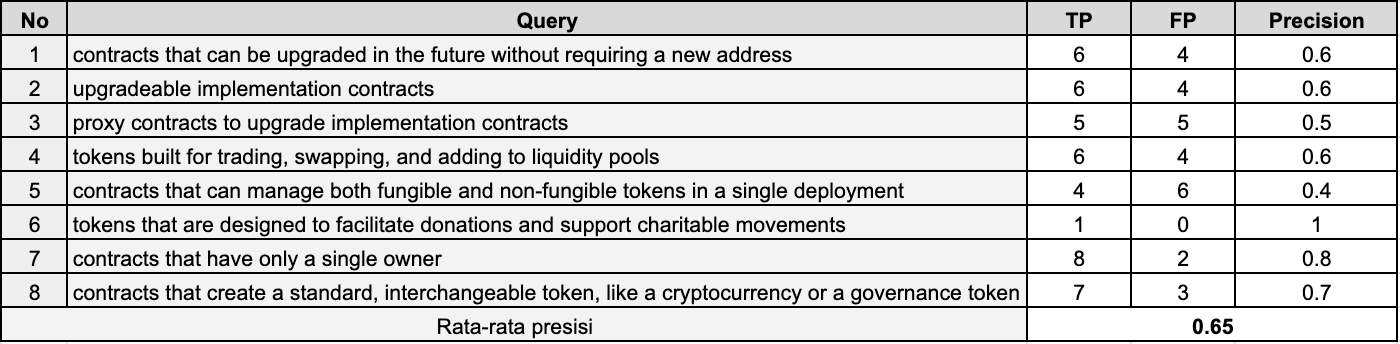
\includegraphics[width=1\textwidth]{resources/chapter-4/data-1-2.png}
	\caption{Hasil Pengujian Sistem Pencarian Berbasis Semantik dari Iterasi Perbaikan dengan Query Bahasa Alami}
	\label{image:pengujian-2}
\end{figure}

\subsubsection{Pengujian Sistem Pencarian Berbasis Semantik dari Iterasi Perbaikan dengan Query Kata Kunci}

Hasil dari pengujian ini dapat dilihat pada Gambar \ref{image:pengujian-3}. Pengujian ini dilakukan dengan menggunakan query berupa kata kunci yang relevan dengan Smart Contract yang ada. Hasil dari pengujian ini menunjukkan rata-rata presisi sebesar 72,5\%, 7,5\% lebih baik dibandingkan dengan menggunakan query bahasa alami.

\begin{figure}[ht]
	\centering
	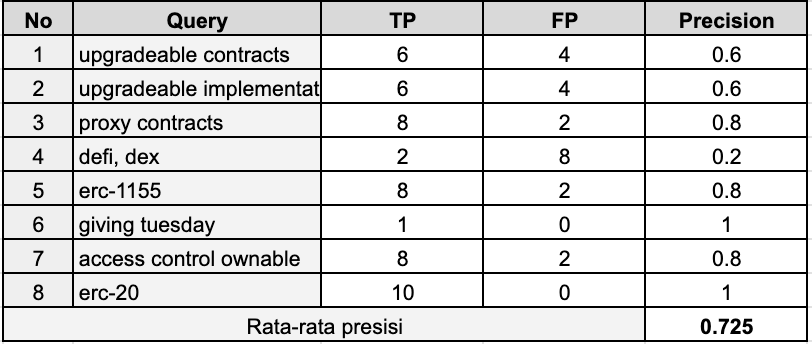
\includegraphics[width=1\textwidth]{resources/chapter-4/data-1-3.png}
	\caption{Hasil Pengujian Sistem Pencarian Berbasis Semantik dari Iterasi Perbaikan dengan Query Kata Kunci}
	\label{image:pengujian-3}
\end{figure}

\subsubsection{Pengujian Sistem Pencarian Berbasis Teks pada Source Code Smart Contract dengan Query Kata Kunci}

Hasil dari pengujian ini dapat dilihat pada Gambar \ref{image:pengujian-4}. Pengujian ini dilakukan dengan menggunakan query berupa kata kunci yang relevan dengan Source Code Smart Contract yang ada. Hasil dari pengujian ini menunjukkan rata-rata presisi sebesar 39\%. Faktor utama dari hasil ini adalah karena sistem hanya melakukan pencarian berbasis sintaks pada Source Code Smart Contract, sehingga tidak dapat memberikan hasil yang relevan dengan konteks yang ada.

\begin{figure}[ht]
	\centering
	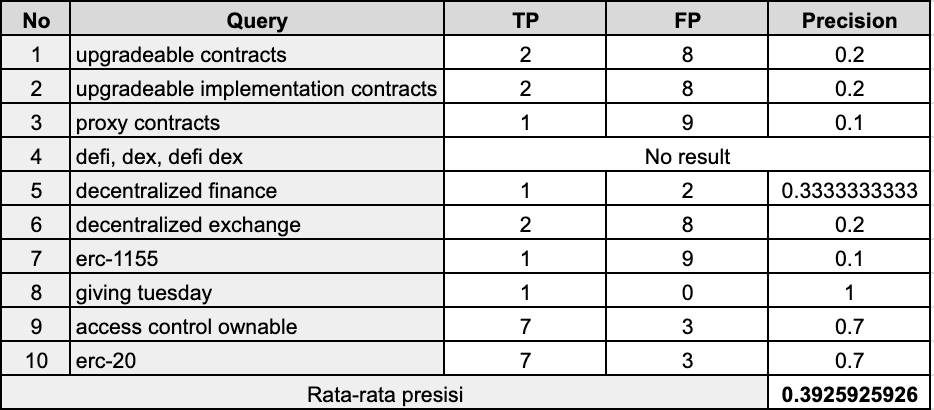
\includegraphics[width=1\textwidth]{resources/chapter-4/data-1-4.png}
	\caption{Hasil Pengujian Sistem Pencarian Berbasis Kata Kunci pada Source Code Smart Contract dengan Query Kata Kunci}
	\label{image:pengujian-4}
\end{figure}

\subsubsection{Pengujian Sistem Pencarian Berbasis Teks pada Deskripsi Semantik dengan Query Kata Kunci}

Hasil dari pengujian ini dapat dilihat pada Gambar \ref{image:pengujian-5}. Pengujian ini dilakukan dengan menggunakan query berupa kata kunci yang relevan dengan deskripsi semantik yang dihasilkan. Hasil dari pengujian ini menunjukkan rata-rata presisi sebesar 49\%. Hasil ini menunjukkan bahwa deskripsi semantik yang dihasilkan dapat memberikan peningkatan relevansi hasil pencarian jika dibandingkan dengan pencarian yang hanya berbasis Source Code.

\begin{figure}[ht]
	\centering
	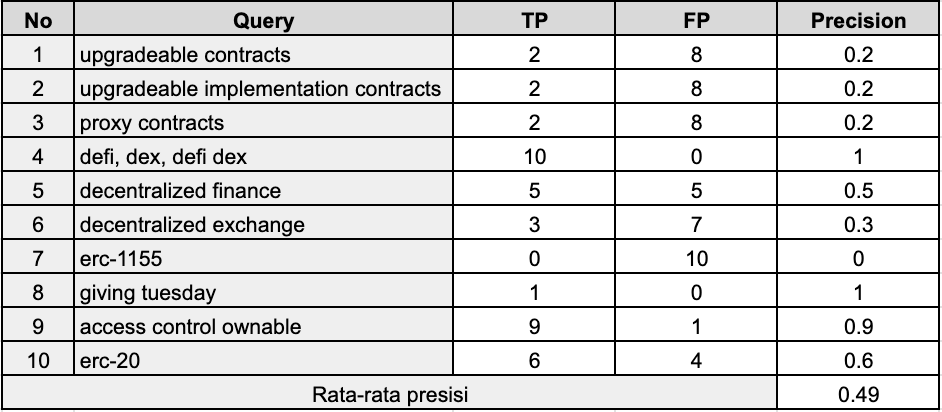
\includegraphics[width=1\textwidth]{resources/chapter-4/data-1-5.png}
	\caption{Hasil Pengujian Sistem Pencarian Berbasis Kata Kunci pada Deskripsi Semantik dengan Query Kata Kunci}
	\label{image:pengujian-5}
\end{figure}

\subsubsection{Pengujian Sistem Pencarian Berbasis Teks pada Deskripsi Semantik dengan Query Bahasa Alami}

Hasil dari pengujian ini dapat dilihat pada Gambar \ref{image:pengujian-6}. Pengujian ini dilakukan dengan menggunakan query berupa bahasa alami yang relevan dengan deskripsi semantik yang dihasilkan pada sistem pencarian berbasis kata kunci. Hasil dari pengujian ini menunjukkan rata-rata presisi sebesar 27,5\%. Hasil ini menunjukkan bahwa query bahasa alami tidak memberikan hasil yang relevan jika digunakan pada sistem pencarian berbasis kata kunci.

\begin{figure}[ht]
	\centering
	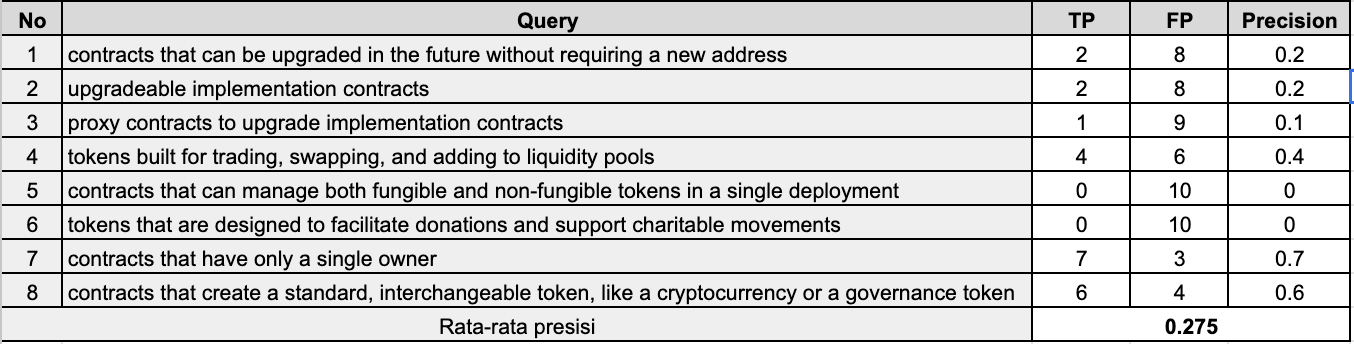
\includegraphics[width=1\textwidth]{resources/chapter-4/data-1-6.png}
	\caption{Hasil Pengujian Sistem Pencarian Berbasis Kata Kunci pada Deskripsi Semantik dengan Query Bahasa Alami}
	\label{image:pengujian-6}
\end{figure}

\subsubsection{Teknis Sistem}
\label{subsec:teknis-sistem}

Terdapat beberapa data yang diambil dari proses enrichment untuk menilai kinerja sistem. Data ini mencakup jumlah token yang digunakan, median dari token yang digunakan, dan waktu yang dibutuhkan untuk melakukan enrichment. Tabel \ref{table:hasil-pengujian-teknis-sistem} menunjukkan hasil pengujian teknis sistem yang dilakukan pada proses enrichment. Data ini diambil dari proses enrichment yang dilakukan pada 118 Smart Contracts yang telah diperkaya dengan deskripsi semantik.

\begin{table}[ht]
	\centering
	\caption{Hasil Pengujian Teknis Sistem}
	\label{table:hasil-pengujian-teknis-sistem}
	\begin{tabular}{|l|c|}
		\hline
		\textbf{Metrik} & \textbf{Nilai} \\ \hline
		Data       	                 & 118         \\ \hline
		Jumlah Token                 & 1.735.909   \\ \hline
		Biaya (GPT 4o mini)          & \$0.23      \\ \hline
		Waktu Proses P50             & 5,56 detik  \\ \hline
		Waktu Proses P99             & 9,41 detik  \\ \hline
		Waktu Proses Embeddings Mean & 0,95 detik \\ \hline
		Waktu Proses Embeddings P50  & 0,375 detik \\ \hline
		Waktu Proses Embeddings P99  & 2,87 detik  \\ \hline
	\end{tabular}
\end{table}
